\documentclass[justified,nobib]{tufte-handout}
\usepackage{microtype}
\usepackage[english,greek]{babel}
\usepackage{inputenc}
\usepackage{graphicx}
\title{Instrumentation Amplifier}
\author{Chris Curro}
\date{\today}
\begin{document}
\selectlanguage{English}
\maketitle
\begin{abstract}
As per the project specification, I designed and implemented an instrumentation
amplifier with a gain of at least 100 over a minimal frequency range of 5~Hz to 
1~kHz. 
\end{abstract}
\section{Design}
\paragraph{}
As can be seen in Figure \ref{schem}, I designed the two-stage amplifier with
three {\sc lf}356 operational amplifiers. I selected this amplifier because of
its wide-band open-loop gain \cite{lf356} to ensure that I met the bandwidth
specification. I decided to design the amplifier with a gain of about 200 so
that even if there were some unexpected issues, I would still be likely to
meet the specification of 100. As per Equation \ref{gaineq}, I selected an $R_2$
value of 100 k$\Omega$ and an $R_1$ value of $1$ k$\Omega$ to result in a gain
of about~200.
\begin{equation}
\label{gaineq}
K = 1 + 2\frac{R_2}{R_1}
\end{equation}
For the sake of simplicity, the remaining resistors, including the load,
were chosen to be 1 k$\Omega$. As a final design consideration, the supply
voltages were selected to be 12 V so that I would have the greatest tolerance to
amplifier saturation with respect to the differential input voltage.
\begin{figure}
\centering
\label{schem}
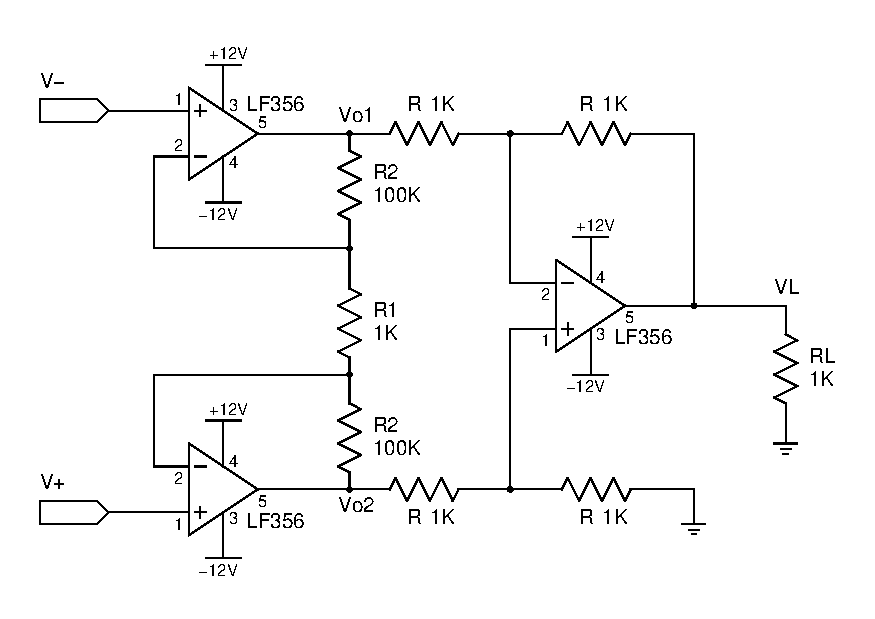
\includegraphics[width=0.9\linewidth,trim=0 .28in 0 .3in,clip=true]{schem.pdf}
\caption{Test schematic for the instrumentation amplifier. A 1 K$\Omega$ load
is included at the output of the final operational amplifier.} 
\end{figure}
%\clearpage
\section{Derivation of Equation \ref{gaineq}}
As practical considerations for the derivation, I will take the ideal
operational amplifier assumption as true, most specifically that the amplifiers
have infinite input impedance and that the two differential inputs are at the
same potential \cite{art}.

First I will consider the gain at the node V$_\textrm{o1}$. By the principle of
superposition I will first assume that V$_{+}$ is 0 V, and then I will assume
that V$_{-}$ is 0 V, and then sum each result to reach the final solution.

\paragraph{Case 1} If V$_{+}$ is at 0 V, then the inverting input to the same
amplifier will also be at 0 V, therefore the bottom half of the circuit
effectively disappears. In this case the top amplifier will act as
a non-inverting amplifier with a gain of:
\begin{equation}
1 + \frac{R_2}{R_1}
\end{equation}
\paragraph{Case 2} If V$_{-}$ is at 0 V, then the inverting input to the same
amplifier will be also be 0 V, while the inverting input to the bottom amplifier
will be at $V_{+}$. In this case the the top amplifier will act as an inverting
amplifier with a gain of:
\begin{equation}
-\frac{R_2}{R_1}
\end{equation}
Combining the two gains by superposition I get:
\begin{equation}
V_\textrm{o1}  = V_{-} \left(1 + \frac{R_2}{R_1}\right)
-V_{+} \frac{R_2}{R_1}
\end{equation}
Similarly, it can be shown that
\begin{equation}
V_\textrm{o2}  = V_{+} \left(1 + \frac{R_2}{R_1}\right)
-V_{-} \frac{R_2}{R_1}
\end{equation}

These two voltages, V$_\textrm{o1}$ and V$_\textrm{o2}$ serve as the two
inputs for the final operational amplifier, which acts as a differential
amplifier with unity gain. Therefore the output voltage of the differential
amplifier is:
\begin{equation}
V_{\mathrm{L}} = V_\textrm{o2} - V_\textrm{o1}  
\end{equation}
Which, with some algebra, becomes:
\begin{equation}
V_{\mathrm{L}} = (V_{+} - V_{-})\left(1 + 2\frac{R_2}{R_1}\right)
\end{equation}
\section{Test Procedure and Results}
\paragraph{Frequency Response} To measure the frequency response of the
instrumentation amplifier, I set V$_{-}$ to be one of the output terminals of
an Agilent 33210A function generator. The other function generator terminal was
tied to the circuit ground. V$_{+}$ was also tied to the circuit ground. I set
the output voltage of the function generator to be 10 mV. I then set the output
waveform to be a sine wave at 5 Hz, and then increased the frequency according
to the scheme set in the specification. All of the following measurements were
made with an Agilient MSO-X 2012A oscilloscope. At each frequency I measured the
peak-to-peak output voltage of the function generator, and the peak-to-peak 
output voltage of the instrumentation amplifier. I divided these quantities to
calculate the gain at each frequency. These results are summarized in Figure
\ref{freqr}.

\begin{figure}
\centering
\label{freqr}
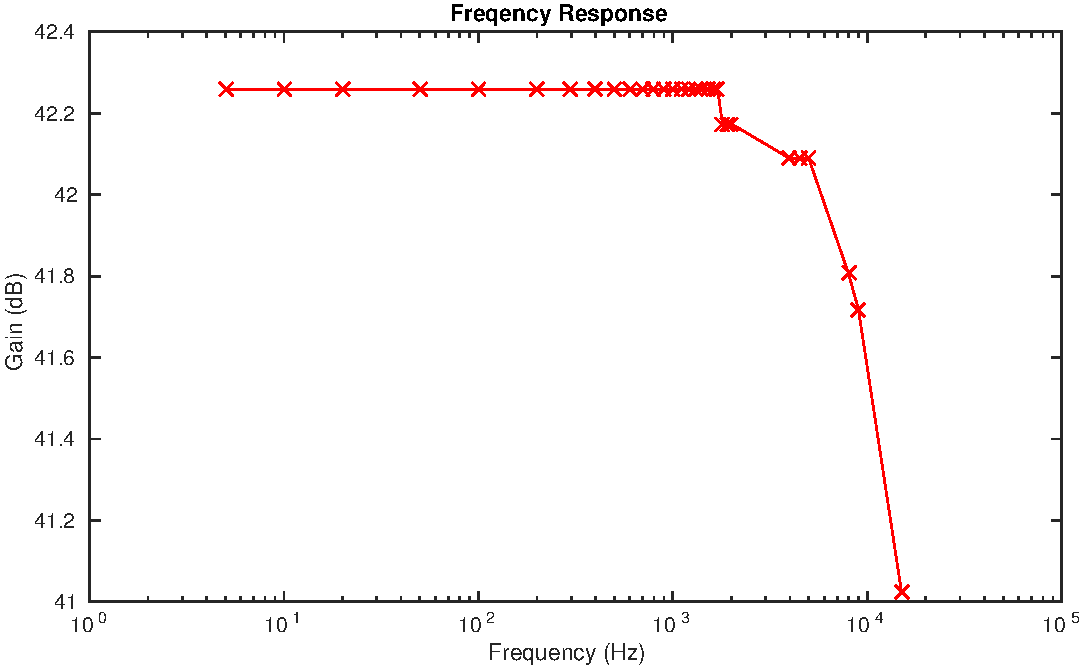
\includegraphics[width=0.9\linewidth]{freq.pdf}
\caption{Frequency response of the instrumentation amplifier}
\end{figure}
\paragraph{Power Consumption}
In order to measure the power consumption for a 100 Hz input signal, I took note
of the voltage and current readouts on the power supply unit. From these (I'm
sure ridiculously inaccurate) measurements, I estimate the power consumption to
be 48 mW.
\paragraph{Common Mode Rejection Ratio} In order to measure the {\sc cmrr} I
connected one terminal of the function generator to both inputs of the
instrumentation amplifier; the other function generator terminal was connected
to ground. I set the output of the function generator to be 1 V, so that even if
the {\sc cmrr} were very high I could still expect to (maybe) see something at
the output of the instrumentation amplifier. Despite this, I discovered that the
the {\sc cmrr} is too high to be measured with my current experimental setup.
Looking back this is to be expected because the {\sc cmrr} of a single 
{\sc lf}356 is 100 dB.

\bibliography{bib}{}
\bibliographystyle{IEEEtran}
\end{document}